\pdfminorversion=4
\documentclass[first=dgreen,second=purple,logo=blueque,finnish]{aaltoslides}

\usepackage[utf8]{inputenc}
\usepackage[T1]{fontenc}
\usepackage{graphicx}
\usepackage{amssymb,amsmath}
\usepackage{url}
\usepackage{lastpage}
\usepackage[english]{babel}

\title{WebSockets / Remote Mouse}

\author[V. Kraemer, Ville Skyttä]{Valter Kraemer, Ville Skyttä}
\institute[ICS]{Department of Information and Computer Science\\
Aalto University, School of Science\\valter.kraemer@aalto.fi, ville.skytta@iki.fi}

\aaltofootertext{WebSockets / Remote Mouse}{Kraemer, Skyttä | 13 Oct 2015}{\insertframenumber/\inserttotalframenumber}

\date{13 October 2015}

\begin{document}

%%%%%%%%%%%%%%%%%%%%%%%%%%%%%%%%%%%%%%%%%%%%%%%%%%%%%%%%%%%%%%%%%%%%%%%%%%%%%%%%%%%%%%%%%%%%%

\aaltotitleframe

%%%%%%%%%%%%%%%%%%%%%%%%%%%%%%%%%%%%%%%%%%%%%%%%%%%%%%%%%%%%%%%%%%%%%%%%%%%%%%%%%%%%%%%%%%%%%

\begin{frame}{WebSockets}

\begin{columns}
\begin{column}{.6\linewidth}
\begin{itemize}
\item Efficient full duplex client-server communications channel
\item Low latency, suitable for real time applications
\item Standardized by IETF (RFC 6455), JavaScript API from W3C
\item Enabler of new type of applications
\item Replaces HTTP abuse, proprietary technologies
\end{itemize}
\end{column}
\begin{column}{.4\linewidth}
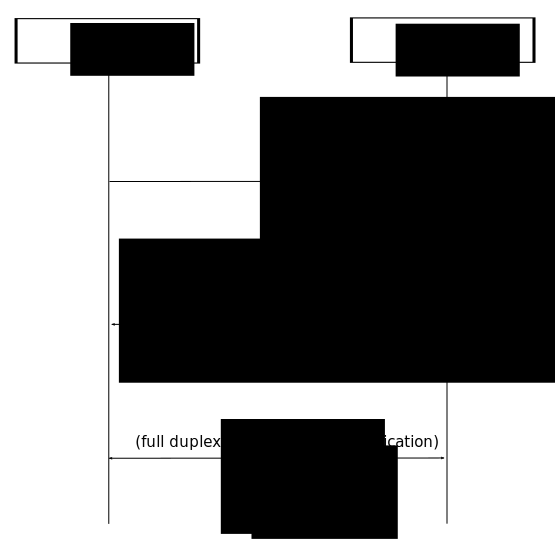
\includegraphics[width=4cm]{ws-handshake}
\end{column}
\end{columns}

\end{frame}

%%%%%%%%%%%%%%%%%%%%%%%%%%%%%%%%%%%%%%%%%%%%%%%%%%%%%%%%%%%%%%%%%%%%%%%%%%%%%%%%%%%%%%%%%%%%%


\begin{frame}{Related Work, State of the Art}

\begin{itemize}
\item New kinds of web applications
\begin{itemize}
\item Multi-screen apps (Bassbouss et al., 2013)
\item Virtual project room (Denoue et al., 2014)
\item Home appliance remote control (Kawazoe et al., 2015)
\end{itemize}
\item Performance related research
\begin{itemize}
\item HTML5 app throughput boundaries (Zhanikeev, 2013)
\item Compression (Anusas-amornkul and Silawong, 2014)
\item Bandwidth estimation with DASH (Cherif et al., 2015)
\end{itemize}
\end{itemize}

\end{frame}

%%%%%%%%%%%%%%%%%%%%%%%%%%%%%%%%%%%%%%%%%%%%%%%%%%%%%%%%%%%%%%%%%%%%%%%%%%%%%%%%%%%%%%%%%%%%%

\begin{frame}{Remote Mouse}

\end{frame}

%%%%%%%%%%%%%%%%%%%%%%%%%%%%%%%%%%%%%%%%%%%%%%%%%%%%%%%%%%%%%%%%%%%%%%%%%%%%%%%%%%%%%%%%%%%%%

\end{document}
